\documentclass[12pt,a4paper]{article}

% Margins.
\setlength{\oddsidemargin}{0in}
\setlength{\evensidemargin}{0in}
\setlength{\headheight}{12pt}
\setlength{\headsep}{42pt}
\setlength{\topmargin}{-54pt}
\setlength{\textwidth}{6.5in}
\setlength{\textheight}{10in}

\usepackage{amsmath}
\usepackage{float}
\usepackage{graphicx}
\usepackage[hyphens]{url}
\usepackage{hyperref}	% Clickable links to figures, references and urls.
\usepackage{datetime}
\usepackage{longtable}
\usepackage{subfigure}

% Links direct to top of figures.
\usepackage[all]{hypcap}

% Drawing.
\usepackage{pgf}
\usepackage{tikz}

% Listings for formatting code.
\usepackage{listings}
\usepackage{textcomp}
% General options.+++
\lstset{breaklines=true, basicstyle=\small\ttfamily, tabsize=4, numbers=left, stepnumber=1, frame=single, showstringspaces=false, upquote=true}
% C++ specific high-lighting. Comments are 50/50 shades of green/black and strings coloured with 60/40 red/black mixture.
\lstset{language=[ISO]C++, commentstyle=\color{green!50!black}, keywordstyle=\color{blue}, stringstyle=\color{red!60!black}}

%opening
\title{\vspace{-3cm}Physics for Engineers\\Class 40\\Magnetic Circuits}
\author{Attique Dawood}
\date{November 28, 2013\\[0.2cm] Last Modified: \today, \currenttime}
\begin{document}
\maketitle
\section{Announcements}
\begin{itemize}
\item Assignment 09 is available.
\end{itemize}
\section{Magnetic Equivalent Circuits}
A simple electromagnet can be made out of a battery and wire wound around something (a pencil would do fine). Commercial electromagnets can range from very small as those in sensitive electronic devices to very large that can lift cars. It is important to know how strong is the magnetic field in the coil, the amount of current required to create such a magnetic field and the amount of flux in the coil.

Magnetic equivalent circuits provide a way of simplifying such problems. The magnetic field of our simple electromagnetic made out of battery, wire and battery is just like that of a natural magnet. Magnetic field lines are spaced very close inside the coil. Recall that $\textbf{B}=\mu\textbf{H}$ where $\mu=\mu_r\mu_0$. For free space $\mu_r=1$ but for iron and steal $\mu_r$ can be as large as 800--1200. What this means is that if we insert a steal or iron core (keeping it insulated from coiled wire) then we can effectively increase the magnetic flux density \textbf{B} a thousandfold! Also since \textbf{B} is increased so is magnetic flux \textbf{inside} the coil. However, this does not mean we have a magical source of increasing magnetic field out of nothing. The extra energy will be supplied by battery. We only increased the value of \textbf{B} keeping the number of turns and the circuit dimensions same as before.

Consider the toroid shown in figure \ref{Toroid-and-equivalent-circuit}. Since the core is made of steel \textbf{B} inside the core will be much greater than in free space. We only consider \textbf{B} and resulting magnetic flux inside the core. To transform such a circuit into equivalent magnetic circuit that will be analogous to electric circuit consider the following conversions:
\begin{itemize}
\item Magnetic flux is the equivalent of electric current. Imagine magnetic flux flowing through the core.
\item Magnetomotive force is the equivalent of voltage source given by $F_{emf}=\oint\limits_{L} \textbf{H}\cdot d\textbf{\textit{l}}=I_{enc}=NI$. This can be obtained by applying Ampere's Law taking the core as path of integration.
\item Electrical resistance is defined as $R=\dfrac{l}{\sigma A}$ where $l$ is the length of resistor, $\sigma$ is conductivity of resistor material and $A$ is cross--sectional area of resistor. Magnetic resistance is known as \textit{reluctance} ($\Re$) and defined in a similar manner replacing $\sigma$ with $\mu$ of core. $\Re=\dfrac{l}{\mu A}$.
\end{itemize}
\section{Exercises}
\noindent\textbf{Question 1 \cite[Example 8.14, page 350]{Sadiku}} The toroidal core of figure \ref{Toroid-and-equivalent-circuit} has $\rho_0$ = 10 cm and a circular cross section with $a=1$ cm. If the core is made of steel ($\mu = 1000\mu_0$) and has a coil with 200 turns, calculate the amount of current that will produce a flux of 0.5 mWb in the core. Assume magnetic flux in the toroid is constant by taking $\rho_0>>a$.\\
\textbf{Answer:} 3.979 A.
\begin{figure}[H]
\centering
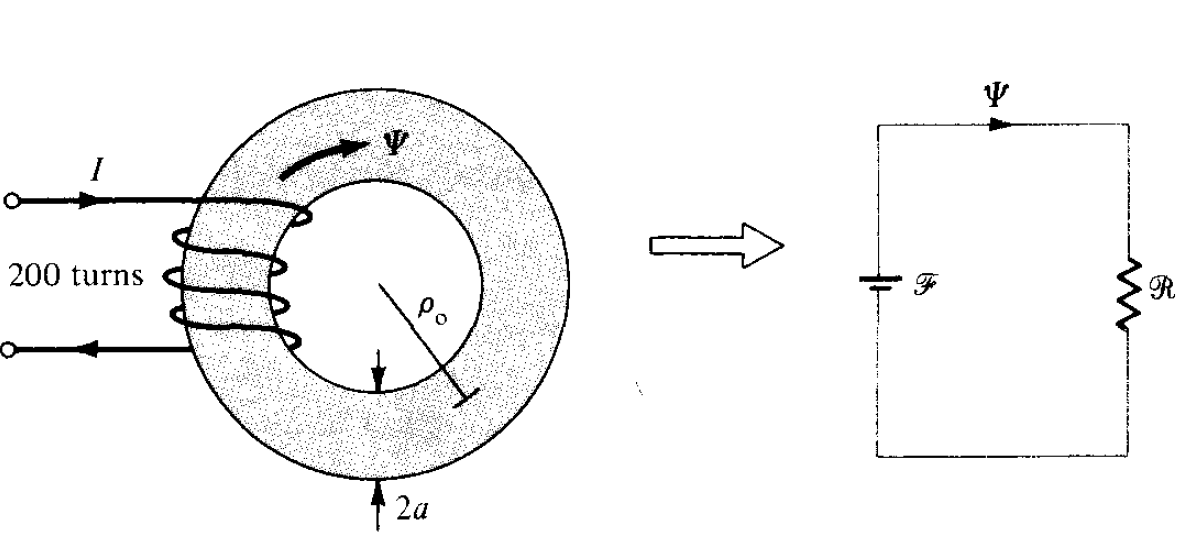
\includegraphics[scale=0.4]{Figure8-26S.png}
\caption{Toroid and equivalent magnetic circuit.}
\label{Toroid-and-equivalent-circuit}
\end{figure}
%\nocite{*}
\bibliographystyle{plain}
\bibliography{PhysicsRef}
\end{document}
